% Options for packages loaded elsewhere
\PassOptionsToPackage{unicode}{hyperref}
\PassOptionsToPackage{hyphens}{url}
\PassOptionsToPackage{dvipsnames,svgnames,x11names}{xcolor}
%
\documentclass[
  letterpaper,
  DIV=11,
  numbers=noendperiod]{scrartcl}

\usepackage{amsmath,amssymb}
\usepackage{iftex}
\ifPDFTeX
  \usepackage[T1]{fontenc}
  \usepackage[utf8]{inputenc}
  \usepackage{textcomp} % provide euro and other symbols
\else % if luatex or xetex
  \usepackage{unicode-math}
  \defaultfontfeatures{Scale=MatchLowercase}
  \defaultfontfeatures[\rmfamily]{Ligatures=TeX,Scale=1}
\fi
\usepackage{lmodern}
\ifPDFTeX\else  
    % xetex/luatex font selection
\fi
% Use upquote if available, for straight quotes in verbatim environments
\IfFileExists{upquote.sty}{\usepackage{upquote}}{}
\IfFileExists{microtype.sty}{% use microtype if available
  \usepackage[]{microtype}
  \UseMicrotypeSet[protrusion]{basicmath} % disable protrusion for tt fonts
}{}
\makeatletter
\@ifundefined{KOMAClassName}{% if non-KOMA class
  \IfFileExists{parskip.sty}{%
    \usepackage{parskip}
  }{% else
    \setlength{\parindent}{0pt}
    \setlength{\parskip}{6pt plus 2pt minus 1pt}}
}{% if KOMA class
  \KOMAoptions{parskip=half}}
\makeatother
\usepackage{xcolor}
\setlength{\emergencystretch}{3em} % prevent overfull lines
\setcounter{secnumdepth}{-\maxdimen} % remove section numbering
% Make \paragraph and \subparagraph free-standing
\ifx\paragraph\undefined\else
  \let\oldparagraph\paragraph
  \renewcommand{\paragraph}[1]{\oldparagraph{#1}\mbox{}}
\fi
\ifx\subparagraph\undefined\else
  \let\oldsubparagraph\subparagraph
  \renewcommand{\subparagraph}[1]{\oldsubparagraph{#1}\mbox{}}
\fi


\providecommand{\tightlist}{%
  \setlength{\itemsep}{0pt}\setlength{\parskip}{0pt}}\usepackage{longtable,booktabs,array}
\usepackage{calc} % for calculating minipage widths
% Correct order of tables after \paragraph or \subparagraph
\usepackage{etoolbox}
\makeatletter
\patchcmd\longtable{\par}{\if@noskipsec\mbox{}\fi\par}{}{}
\makeatother
% Allow footnotes in longtable head/foot
\IfFileExists{footnotehyper.sty}{\usepackage{footnotehyper}}{\usepackage{footnote}}
\makesavenoteenv{longtable}
\usepackage{graphicx}
\makeatletter
\def\maxwidth{\ifdim\Gin@nat@width>\linewidth\linewidth\else\Gin@nat@width\fi}
\def\maxheight{\ifdim\Gin@nat@height>\textheight\textheight\else\Gin@nat@height\fi}
\makeatother
% Scale images if necessary, so that they will not overflow the page
% margins by default, and it is still possible to overwrite the defaults
% using explicit options in \includegraphics[width, height, ...]{}
\setkeys{Gin}{width=\maxwidth,height=\maxheight,keepaspectratio}
% Set default figure placement to htbp
\makeatletter
\def\fps@figure{htbp}
\makeatother

\KOMAoption{captions}{tableheading}
\makeatletter
\@ifpackageloaded{caption}{}{\usepackage{caption}}
\AtBeginDocument{%
\ifdefined\contentsname
  \renewcommand*\contentsname{Table of contents}
\else
  \newcommand\contentsname{Table of contents}
\fi
\ifdefined\listfigurename
  \renewcommand*\listfigurename{List of Figures}
\else
  \newcommand\listfigurename{List of Figures}
\fi
\ifdefined\listtablename
  \renewcommand*\listtablename{List of Tables}
\else
  \newcommand\listtablename{List of Tables}
\fi
\ifdefined\figurename
  \renewcommand*\figurename{Figure}
\else
  \newcommand\figurename{Figure}
\fi
\ifdefined\tablename
  \renewcommand*\tablename{Table}
\else
  \newcommand\tablename{Table}
\fi
}
\@ifpackageloaded{float}{}{\usepackage{float}}
\floatstyle{ruled}
\@ifundefined{c@chapter}{\newfloat{codelisting}{h}{lop}}{\newfloat{codelisting}{h}{lop}[chapter]}
\floatname{codelisting}{Listing}
\newcommand*\listoflistings{\listof{codelisting}{List of Listings}}
\makeatother
\makeatletter
\makeatother
\makeatletter
\@ifpackageloaded{caption}{}{\usepackage{caption}}
\@ifpackageloaded{subcaption}{}{\usepackage{subcaption}}
\makeatother
\ifLuaTeX
  \usepackage{selnolig}  % disable illegal ligatures
\fi
\usepackage{bookmark}

\IfFileExists{xurl.sty}{\usepackage{xurl}}{} % add URL line breaks if available
\urlstyle{same} % disable monospaced font for URLs
\hypersetup{
  pdftitle={Table 1 and Figure 1},
  colorlinks=true,
  linkcolor={blue},
  filecolor={Maroon},
  citecolor={Blue},
  urlcolor={Blue},
  pdfcreator={LaTeX via pandoc}}

\title{Table 1 and Figure 1}
\author{}
\date{}

\begin{document}
\maketitle

\subsection{Table 1}\label{table-1}

This table summaries characteristics of the data set across countries
which had a conflict and those that did not

\begin{longtable}[]{@{}
  >{\raggedright\arraybackslash}p{(\columnwidth - 6\tabcolsep) * \real{0.3855}}
  >{\raggedright\arraybackslash}p{(\columnwidth - 6\tabcolsep) * \real{0.2048}}
  >{\raggedright\arraybackslash}p{(\columnwidth - 6\tabcolsep) * \real{0.2048}}
  >{\raggedright\arraybackslash}p{(\columnwidth - 6\tabcolsep) * \real{0.2048}}@{}}
\toprule\noalign{}
\begin{minipage}[b]{\linewidth}\raggedright
\end{minipage} & \begin{minipage}[b]{\linewidth}\raggedright
Conflict Present
\end{minipage} & \begin{minipage}[b]{\linewidth}\raggedright
Conflict Absent
\end{minipage} & \begin{minipage}[b]{\linewidth}\raggedright
All countries
\end{minipage} \\
\midrule\noalign{}
\endhead
\bottomrule\noalign{}
\endlastfoot
& (N=42) & (N=144) & (N=186) \\
GDP (in 1000s) & & & \\
Median (IQR) & 0.62 (0.4 - 1.7) & 2.5 (0.8 - 11.2) & 1.8 (0.6 - 6.5) \\
Missing & 3 (7.1\%) & 4 (2.8\%) & 7 (3.8\%) \\
Age Dependency Ratio & & & \\
Median (IQR) & 84 (59.9 - 94.8) & 60 (48.4 - 78.3) & 63 (49.5 - 84.7) \\
Male Education Level & & & \\
Median (IQR) & 5.5 (3.7 - 6.8) & 7.9 (5.4 - 10.6) & 7.1 (4.9 - 10.1) \\
Missing & 1 (2.4\%) & 0 (0\%) & 1 (0.5\%) \\
Urban Population (\%) & & & \\
Median (IQR) & 27 (19.3 - 36.8) & 28 (14.7 - 40) & 28 (15.4 - 39.7) \\
Missing & 1 (2.4\%) & 0 (0\%) & 1 (0.5\%) \\
Years with Conflict (2000-2008) & & & \\
Median (IQR) & 9.0 (7.2 - 9) & 0 (0 - 1) & 0 (0 - 4) \\
Years with Conflict (2009-2017) & & & \\
Median (IQR) & 9.0 (7 - 9) & 0 (0 - 1) & 0 (0 - 4) \\
Total Deaths (Yearly) & & & \\
Median (IQR) & 2.8 (1.2 - 6.6) & 0 (0 - 0.1) & 0.034 (0 - 0.8) \\
Maternal Deaths (Yearly) & & & \\
Median (IQR) & 13 (3.8 - 32.4) & 2.8 (0.6 - 10.3) & 3.7 (1 - 18.1) \\
Missing & 0 (0\%) & 3 (2.1\%) & 3 (1.6\%) \\
Neonatal Deaths (Yearly) & & & \\
Median (IQR) & 1.4 (0.8 - 2) & 0.58 (0.2 - 1.3) & 0.71 (0.3 - 1.5) \\
Missing & 0 (0\%) & 1 (0.7\%) & 1 (0.5\%) \\
Infant Deaths (Yearly) & & & \\
Median (IQR) & 2.4 (1.1 - 3.8) & 0.93 (0.3 - 2.1) & 1.1 (0.5 - 2.7) \\
Missing & 0 (0\%) & 1 (0.7\%) & 1 (0.5\%) \\
Under 5 Deaths (Yearly) & & & \\
Median (IQR) & 3.3 (1.3 - 5.2) & 1.1 (0.4 - 2.7) & 1.3 (0.5 - 3.7) \\
Missing & 0 (0\%) & 1 (0.7\%) & 1 (0.5\%) \\
\end{longtable}

\subsection{Figure 1}\label{figure-1}

This figure shows countries which experienced increasing maternal
mortality

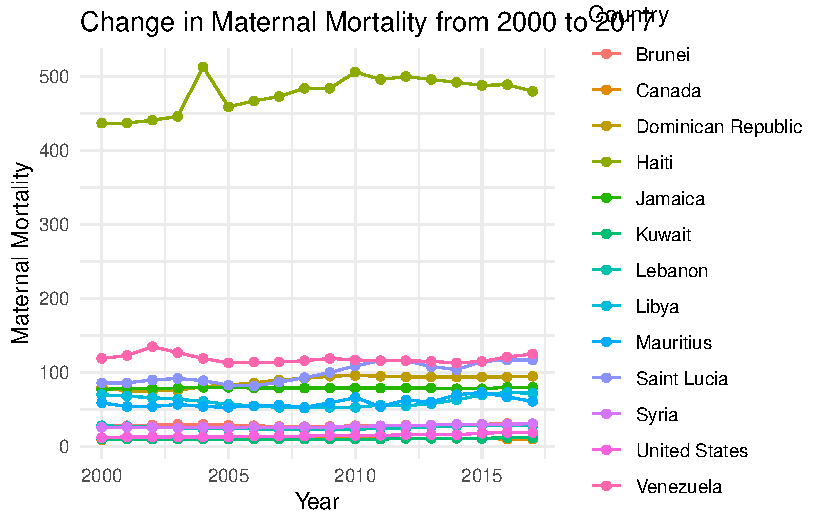
\includegraphics{Tab1_Fig_1_files/figure-pdf/unnamed-chunk-2-1.pdf}

The \texttt{echo:\ false} option disables the printing of code (only
output is displayed).



\end{document}
